\title{Homework 1: Diagnostic}

\author{Jean Salac (salac@uchicago.edu)}

\documentclass[letterpaper,12pt]{article}
\usepackage[letterpaper, portrait, margin = 0.5 in]{geometry}
\usepackage{graphicx}
\graphicspath{{images/}}
\usepackage{enumitem}

\begin{document}
\maketitle
\begin{center}
GitHub Repo: https://github.com/jeansalac/ml-ppol \\
Collaborator: Yuliana Zamora
\end{center}

\section{Data Acquisition and Analysis}
\textbf{Requests per Month:} \\
\begin{center}
\begin{tabular}{ |c|c|c| } 
 \hline
 \textbf{Requests} & \textbf{Mean Requests per Month} & \textbf{Standard Deviation} \\ 
 \hline
 Graffiti Removal & 9398.25 & 135.37 \\ 
 \hline
 Vacant and Abandoned Buildings & 305.5 & 72.35 \\ 
 \hline
 Lights out in Alleys & 2324.67 & 308.24 \\
 \hline
\end{tabular}
\end{center}

\vspace{10mm}

\noindent \textbf{Number of Graffiti Removal Requests Every Month in 2017} \\
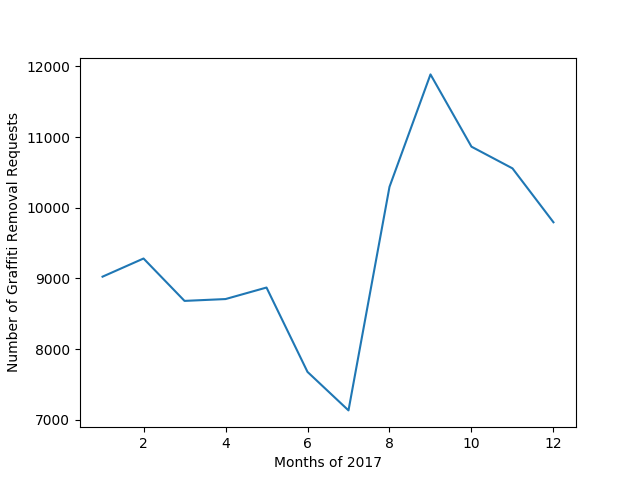
\includegraphics[scale=1]{grafovertime.png}

\noindent \textbf{Number of Vacant and Abandoned Buildings Reported Every Month in 2017} \\
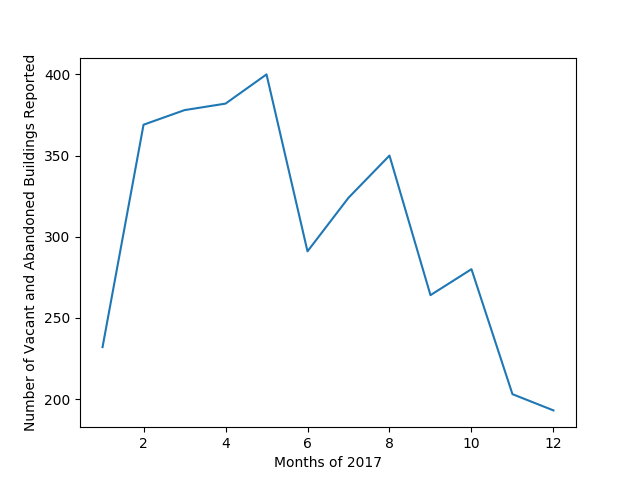
\includegraphics[scale=.9]{buildovertime.png}

\noindent \textbf{Number of Alley Lights Out Reported Every Month in 2017} \\
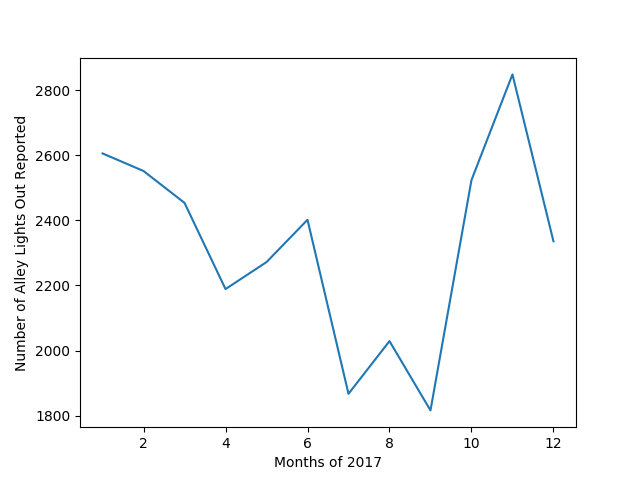
\includegraphics[scale=.9]{alleysovertime.png} \\

\newpage

\noindent \textbf{Number of Graffiti Removal Requests for Each Community Area in 2017} \\
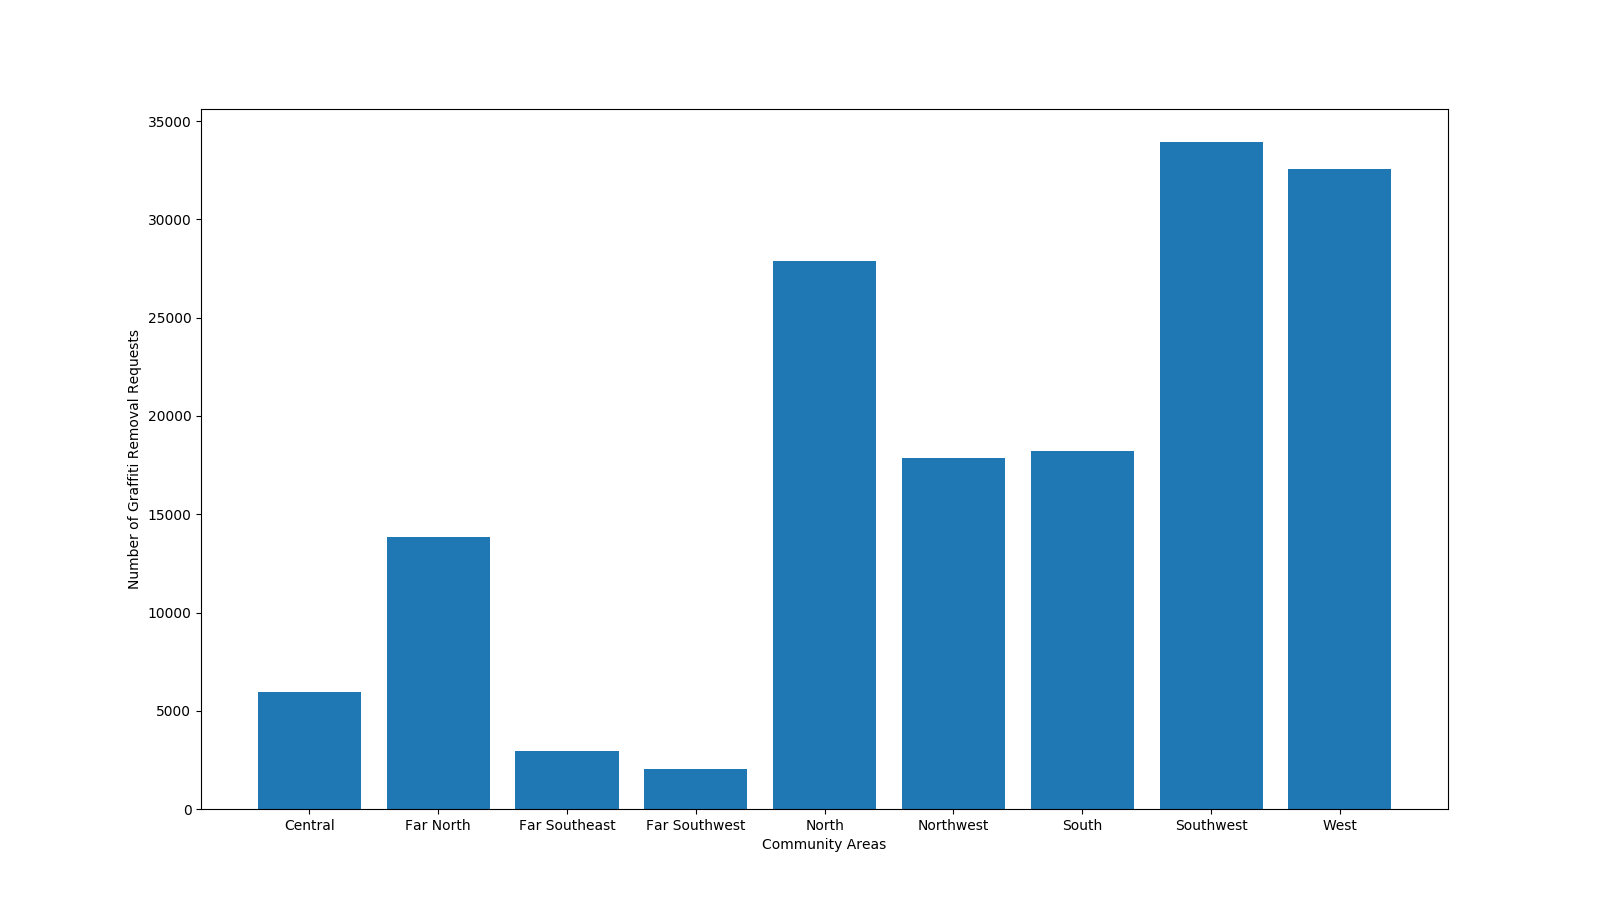
\includegraphics[scale=.46]{grafovercommunity.png}

\noindent \textbf{Number of Vacant and Abandoned Buildings Reported for Each Community Area in 2017} \\
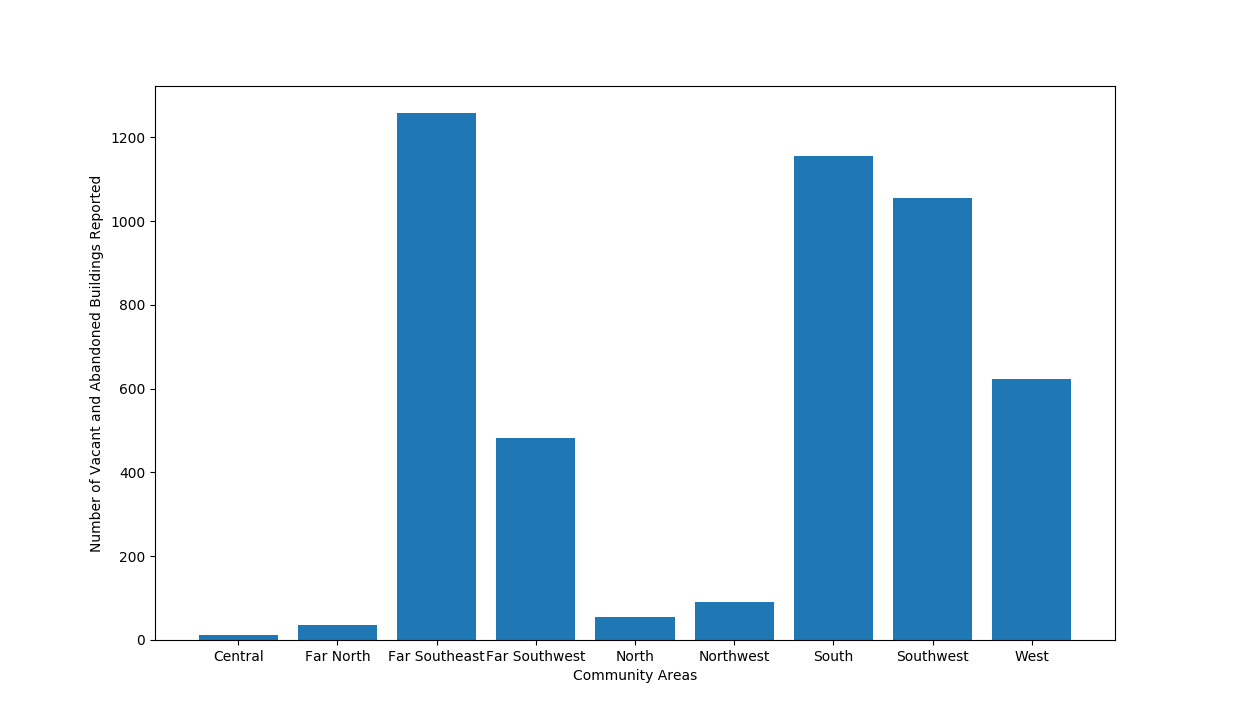
\includegraphics[scale=.6]{buildovercommunity.png}

\newpage

\noindent \textbf{Number of Alley Lights Out Reported for Each Community in 2017} \\
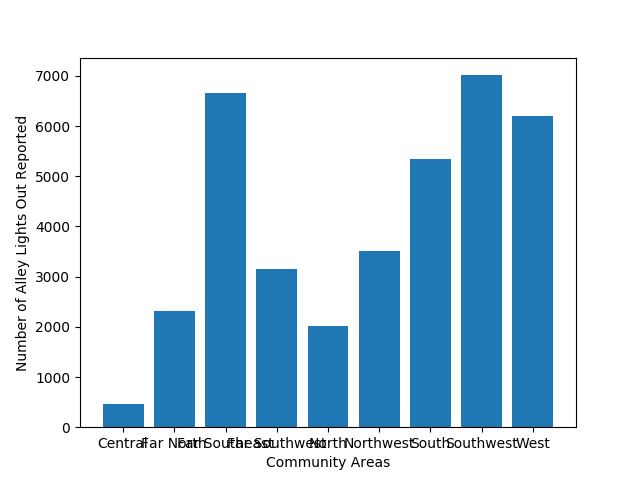
\includegraphics[scale=.6]{alleysovercommunity.png}

\noindent \textbf{Response Time for Graffiti Reported} \\
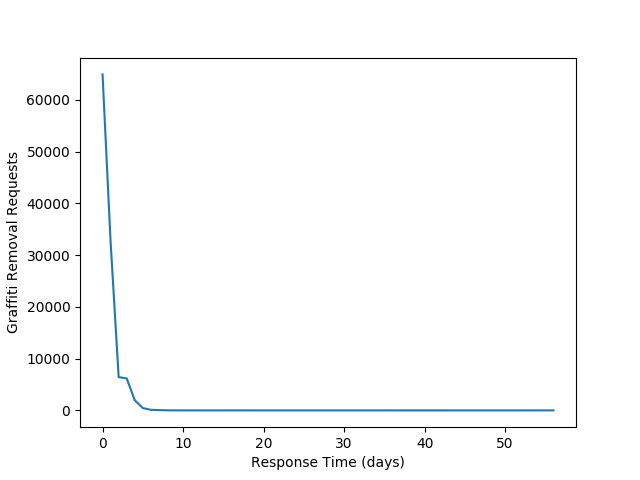
\includegraphics[scale=1]{responseovergraf.png}

\newpage

\noindent \textbf{Response Time for Alley Lights Out Reported} \\
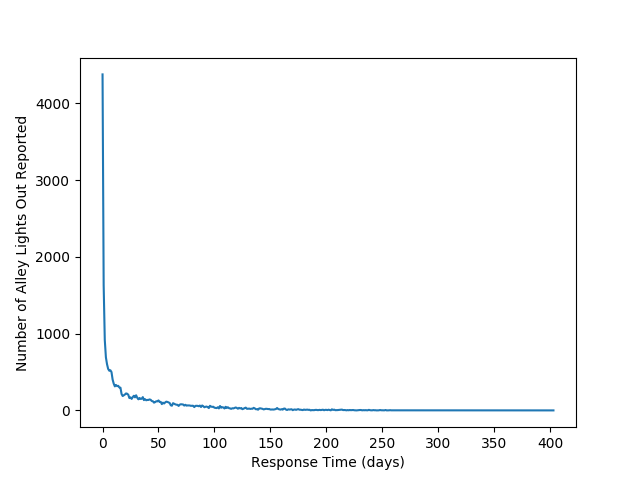
\includegraphics[scale=1]{responseoveralleys.png}

\noindent \textbf{Interesting Things Learned from the Data}
\begin{enumerate}
\item The number of graffiti removal requests and alley lights out reported dip in the summer months, while the number of vacant and abandoned buildings reported rise in the summer.
\item The greatest graffiti removal requests come from the North Side, Southwest Side, and West Side. This could be either a reflection of the amount of graffiti in those communities or the community's tolerance for graffiti.
\item The greatest number of vacant and abandoned buildings reported come from the Far Southeast, South, Southwest communities.
\item The greatest number of the alley lights reported are from the Far Southeast, South, and Southwest communities.
\item Most of the requests for graffiti removal were responded to in under 10 days, while most of the requests for the alley lights out reported were responded to in under 50 days. This discrepancy could be because it may be easier to clean up graffiti than to identify and replace which alley lights are out.
\end{enumerate}

\section{Data Augmentation and APIs}

\section{Probability}
\begin{itemize}
\item Zip code for 3600 W Roosevelt Ave: 60624
\item Zip codes for Uptown: 60613 and 60640
\item The values came from the number of requests for the zip code 60624 over all the years.
\end{itemize}

\begin{enumerate}[label = \Alph*]
\item \textbf{Probabilities of Requests}
\begin{itemize}
\item Number of Graffiti Removal Requests (G) = 3274
\item Number of Vacant and Abandoned Buildings Requests (B) = 3069
\item Number of Lights Out in Alleys Requests (L)= 3244
\item Total Number of Requests = 9587
\item $P(G) = \frac{3274}{9587} \times 100 = 34.15\%$
\item $P(B) = \frac{3069}{9587} \times 100 = 32.01\%$
\item $P(L) = \frac{3244}{9587} \times 100 = 33.84\%$
\item Thus, graffiti removal is the most likely request from Garfield Park.
\end{itemize}

\item \textbf{Garfield vs Uptown - with raw data}
\begin{itemize}
\item Number of Graffiti Removal Requests from Garfield Park (GP) = 3274
\item Number of Graffiti Removal Requests from Uptown (U)= 19182+17653=36835
\item Total number of Graffiti Removal Requests = 40109
\item $P(GP) = \frac{3274}{40109} \times 100 = 8.16 \%$
\item $P(U) = \frac{36835}{40109} \times 100 = 98.14 \%$
\item A graffiti removal request is $\frac{36835}{3274} = 11.25$ times more likely to be from Uptown than Garfield Park.
\end{itemize}

\item \textbf{Garfield vs Uptown - without raw data}
\begin{itemize}
\item $P(Garfield | Graffiti) = \frac{100}{100+160} \times 100 = 36.46 \%$
\item $P(Uptown | Graffiti) = \frac{160}{100+160} \times 100 =61.54 \%$
\item A graffiti removal request is $\frac{160}{100} = 1.6$ times more likely to be from Uptown than Garfield Park.
\end{itemize}

\end{enumerate}
\end{document}